\section{Theoretical Linguistics}
    
    
\section{Definition}
    Language is a system of conventional symbols (spoken, written, or signed) that enables members of a community to communicate ideas, experiences, and intentions.
    Encyclopedia Britannica
    
    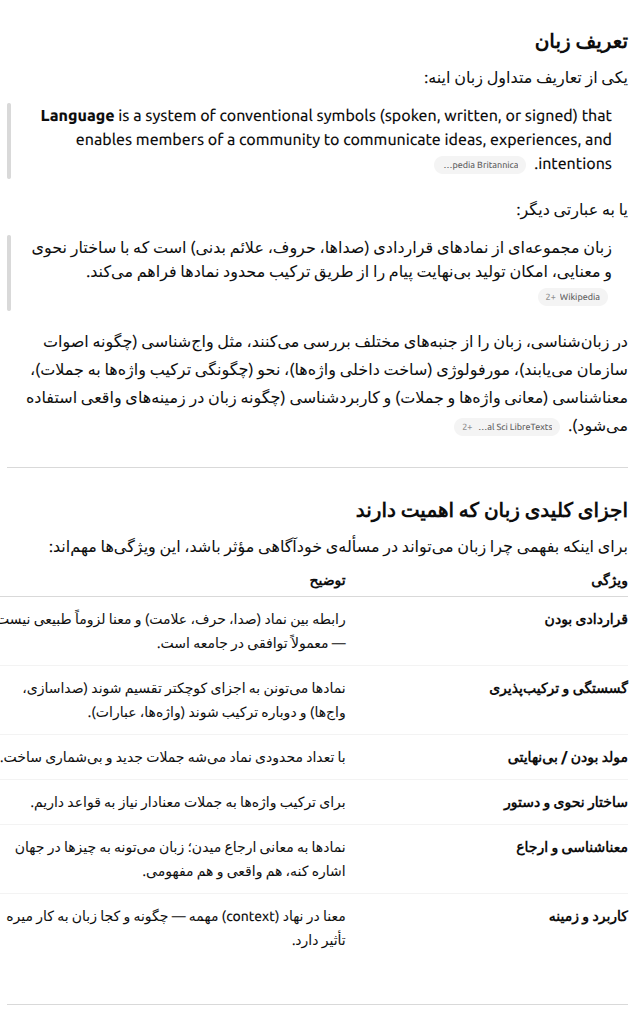
\includegraphics[width=1\linewidth]{language_definition.png}
    
    
    \subsection{Phonetics}
    
    
    \subsection{Phonology}
    
    
    \subsection{Morphology}
    
    
    \subsection{Syntax}
    
    
    \subsection{Semantics}
    
    
    \subsection{Pragmatics}


\section{Applied Linguistics}


\section{Interdiciplinary}
    
    
    \subsection{Psycholinguistics}
    
    
    \subsection{Sociolinguistics}
    
    
    \subsection{Historical Linguistics}
    
    
    \subsection{Anthropological Linguistics}
    
    
    \subsection{Computational Linguistics}
    
    
    \subsection{Cognitive Linguistics}
    
    
    \subsection{Corpus Linguistics}
    
    
    \subsection{Biolinguistics}
        How does language ability roots in body and genetics
        Noam Chomsky "Language Faculty"
    
    
    \subsection{Neurolinguistics}
    
    
\section{Cognitive Neuroscience of Language}


\section{Language Acquisition}
    \url{https://en.wikipedia.org/wiki/Language_acquisition}
    
    \chapter{Biological perspective}
\url{https://www.amazon.de/-/en/dp/0199284776/?coliid=I2ZFZ3O9PPZ6RM&colid=662UPZCH1AIN&psc=1&ref_=list_c_wl_lv_ov_lig_dp_it}
    
\url{https://www.amazon.de/-/en/dp/B08B1HS3XZ/?coliid=I2QQPO9D6WJT6H&colid=662UPZCH1AIN&psc=0&ref_=list_c_wl_lv_ov_lig_dp_it}
    \section{Computational linguistic}